\section{Anforderungsspezifikation}
\subsection{Allgemeine Beschreibung}
Im generellen sind zwei Anwendungsszenarien denkbar:
\begin{itemize}
	\item VPN-Client
	\item VPN-Gateway
\end{itemize}
\medskip
Dabei ist der VPN-Client eine \textbf{Muss}-Anforderung und der VPN-Gateway eine \textbf{Kann}-Anforderung.
\medskip
\subsubsection{VPN-Client}
Die Applikation wird von einem Standard-Nutzer verwendet. Dieser soll VPN Tunnels zu Gateways konfigurieren können und die Tunnels starten und stoppen. Die Konfigurationsmöglichkeiten sind beschränkt, als Richtwert wird der strongSwan Android Client verwendet.\\


\subsubsection{VPN-Gateway}
Der Gateway ist auf Systemadministratoren ausgerichtet. Es soll möglich sein per grafischem Interface strongSwan zu konfigurieren und Tunnels einzurichten, welche als Gateway genutzt werden. 

\subsection{Use Case}
\subsubsection{Aktoren und Stakeholder}
\begin{table}[H]
\centering
    \begin{tabular}{|p{3cm}|p{9cm}|}
    \hline
    \rowcolor{lightblue}
    Aktor & Tätigkeit   \\ \hline
	User  & 
			\begin{itemize}
			\item Konfiguriert VPN-Tunnel als Client
    		\item Startet und stoppt VPN-Tunnel
		\end{itemize}	
	\\ \hline
	Administrator & 
			\begin{itemize}
			\item Konfiguriert VPN-Tunnel als Gateway
    		\item Startet und stoppt VPN-Tunnel
		\end{itemize}	
	\\ \hline
	\end{tabular}
    \caption[Aktoren und Stakeholder]{Aktoren und Stakeholder}
\end{table}

\subparagraph{hallo welt}


\subsubsection{Use Case Diagramm}
\begin{figure}[H]
\centering
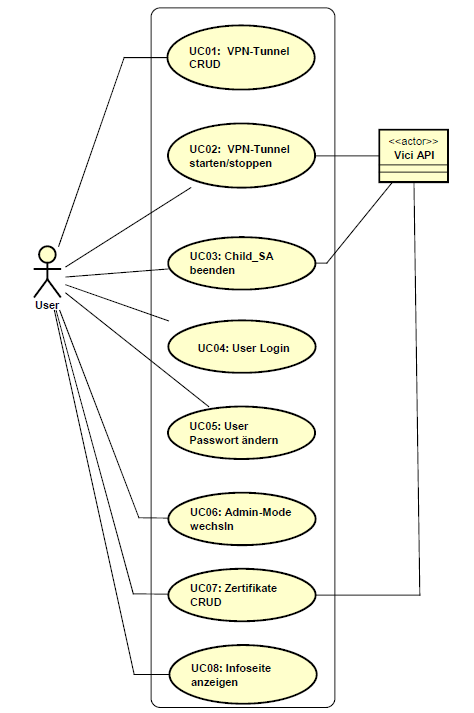
\includegraphics[width=420pt]{images/strongMan_usecase.png}
\caption[Use Case Diagramm]{Use Case Diagramm}
\end{figure}


\subsubsection{Use Cases Brief}
Alle hier definierten Use Cases haben auch ein entsprechendes Mockup im Anhang.
\paragraph{UC01: VPN-Tunnel CRUD}\mbox{} \\
Der User kann einen VPN-Tunnel erfassen / konfigurieren. Dabei hat er eine Auswahl von verschiedenen vordefinierten Tunneltypen. Jeder Tunneltyp hat eigene Konfigurationsfelder, die der User ausfüllen muss. Die Tunnel-Übersichtsseite stellt die Hauptseite der Applikation dar. Dort können die Tunnels bearbeitet und gelöscht werden.

\paragraph{UC02: VPN-Tunnel starten/stoppen}\mbox{} \\
Der User kann einen erfassten VPN-Tunnel starten und stoppen. Dabei wird die Konfiguration über die Vici API geladen. Falls ein VPN-Tunnel nicht aufgebaut werden kann, soll eine passende Fehlermeldung angezeigt werden. 

\paragraph{UC03: Child\_SA beenden}\mbox{} \\
Jeder VPN-Tunnel kann mehrere Child\_SA enthalten. Dieser werden in der Hauptseite angezeigt und können vom User beendet werden. Dieser Use Case interagiert mit der VICI Schnittstelle.

\paragraph{UC04: User Login}\mbox{} \\
Der User loggt sich zu Beginn beim Webseiten Aufruf mit einem Passwort ein. Es existiert dabei nur ein User mit Passwort.

\paragraph{UC05: User Passwort ändern}\mbox{} \\
Sobald der User eingeloggt ist, hat er die Möglichkeit, sein Passwort zu ändern. Dabei gibt er sein altes Passwort einmal und sein neues Passwort zweimal ein.

\paragraph{UC06: Admin-Mode wechseln}\mbox{} \\
Das Userinterface unterscheidet zwischen zwei Modis: User- \& Admin-Mode. Der Mode kann durch einem Klick auf einen Button gewechselt werden. Der Admin-Mode stellt einige Gateway-spezifische Funktionalitäten zusätzlich zur Verfügung, welche der User zur einfacheren Bedienung nicht sieht.

\paragraph{UC07: Zertifikate CRUD}\mbox{} \\
Dem User wird eine Zertifikatsverwaltung zur Verfügung gestellt. Er kann Zertifikate und Private Key's in den gängigen Formaten uploaden, anschauen, updaten (Passwort ändern) und wieder löschen. Die Dateien können mit einem Passwort verschlüsselt sein. Dieser Use Case interagiert unter Umständen mit der VICI Schnittstelle.

\paragraph{UC08: Infoseite anzeigen}\mbox{} \\
Die Infoseite zeigt dem eingeloggten User verschieden Informationen über das installierte System wie Charon Version, installierte Plugins usw.

\subsubsection{Definition Konfigurationsmöglichkeiten UC01}
\paragraph{VPN-Client}\mbox{} \\
Folgende Tunneltypen müssen unterstützt werden:
\begin{itemize}
	\item IKEv2	Zertifikat	
	\item IKEv2 EAP (Benutzername/Passwort)
	\item IKEv2	Zertifikat + EAP (Benutzername/Passwort)
	\item IKEv2	EAP-TLS (Zertifikat)
\end{itemize}

\paragraph{Eingabefelder}
\begin{table}[H]
	\centering
    \begin{tabular}{|p{3cm}|p{7.5cm}|p{6cm}|}
    \hline    
    \rowcolor{lightblue}
	Name & swanclt & vici \\ \hline   
	Profilname & connections.<conn> & <IKE\_SA config name> \\ \hline
	Typ & "Verbindungsarten" & "Verbindungsarten" \\ \hline
	Gateway & connections.<conn>.remote\_addrs & remote-host \\ \hline
	EAP Username & 
connections.<conn>.local<suffix>.eap\_id (Ref: secrets.eap<suffix>.id<suffix>)& <IKE>.remote-eap-id \\ \hline
	EAP Passwort & secrets.eap<suffix>.secret &<secret>.data \\ \hline
	Gateway-Port & connections.<conn>.remote\_port & <IKE>.remote-port \\ \hline
	CA-Zertifikat & connections.<conn>.remote<suffix>.cacerts & \\ \hline
	User-Zertifikat & connections.<conn>.local<suffix>.certs & \\ \hline
	\end{tabular}
    \caption[Eingabefelder VPN-Client]{Eingabefelder VPN-Client}
\end{table}


\paragraph{VPN-Gateway}\mbox{} \\




